\section{Results}
\begin{table}[H]
    \centering
    \caption{Tabular overview of the numerical convergence towards the analytical values committed by the 2x2 Ising model for increasing MCS. Here $\beta_0 = 1$.}
    \begin{tabular}{l|l|l|l|l}
    \hline
         MCS & $\langle E \rangle _{\beta_0}$ & $\langle |M| \rangle _{\beta_0}$ & $C_V$ & $\mathcal{X}$\\
         \hline
         100 & -1.94000 & 0.97500& 0.46560 & 0.08750 \\
         1000 & -1.98800&  0.99900& 0.01598 & 0.00391 \\
         10000 & -1.99340&  0.99755 & 0.05253 & 0.00807 \\
         100000 & -1.99552&  0.99853& 0.03571 & 0.00433 \\
         1000000 & -1.99585&  0.99851& 0.03313 & 0.00427\\
         10000000 & -1.99600&  0.99869&  0.03131 & 0.00395\\
         \hline
         Analytical value &-1.99598 & 0.99866 & 0.03203 & 0.00401\\
         \hline
    \end{tabular}
    
    \label{tab:2x2compare}
\end{table}

\begin{table}[H]
    \centering
    \caption{Tabular overview of the numerical errors in the studied quantities and their associated number of Monte Carlo sweeps.}
    \begin{tabular}{l|l|l|l|l}
    \hline
    MCS & $\epsilon\ (\langle E \rangle)$ & $\epsilon\ (\langle |M|\rangle)$ & $\epsilon\ (C_V)$ & $\epsilon\ (\mathcal{X})$\\
    \hline
         10$^6$ & 6.51$\cdot 10^{-5}$ & 1.50$\cdot10^{-4}$ & 3.43$\cdot10^{-2}$ & 6.48$\cdot10^{-2}$  \\
         10$^7$ & 1.00$\cdot10^{-5}$ & 3.00$\cdot10^{-5}$ & 2.25$\cdot10^{-2}$ & 1.50$\cdot10^{-2}$  
    \end{tabular}
    
    \label{tab:my_label}
\end{table}

Table \ref{tab:2x2compare} provides a tabular overview of how the numerical implementation of the Metropolis algorithm computes expectation values for the different physical quantities of interest for the 2x2 Ising model which converge towards the analytical value with an increasing number of Monte Carlo sweeps. Observe that for one million sweeps, there is a very good agreement between the numerical and analytical value for the mean energy $\langle E \rangle$ and the mean absolute magnetization $\langle |M| \rangle$. The precision increases further for ten million sweeps. However, the relative errors in the computed values of $C_V$ and $\mathcal{X}$ remain a few magnitudes of order larger. The reason the two quantities seem computationally sensitive is due to the propagation of statistical error as they are functions defined by the variables $E$ and $|M|$ which both carry their own relative error. 


%Oppgave 4d
\begin{figure}[H]
		\centering
		\begin{subfigure}{0.48\linewidth}
			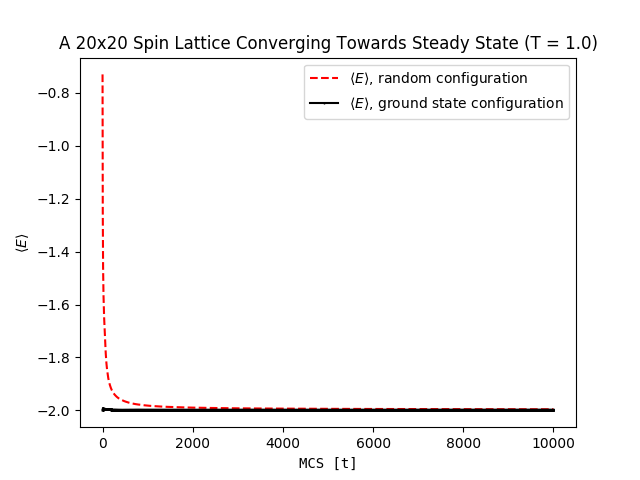
\includegraphics[width=1.08\linewidth]{Figure/20x20_Econvergence_1.0.png}
			\caption{$k_B T$ = 1.0 J}
		\end{subfigure}
		\begin{subfigure}{0.48\linewidth}
			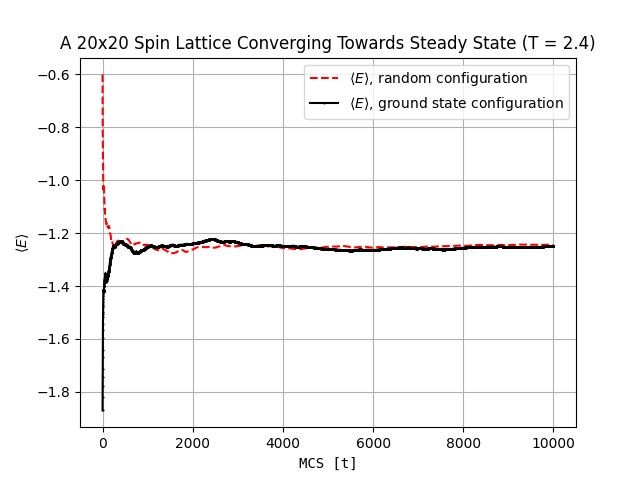
\includegraphics[width=1.08\linewidth]{Figure/20x20_Econvergence_2.4.png}
			\caption{$K_B T $ = 2.4 J}
		\end{subfigure}
		\caption{Convergence of mean energy as a function of Monte Carlo Sweeps (MCS).}
		\label{econvergence}
	\end{figure}
	
Figure \ref{econvergence} shows the equilibration period for a 20x20 lattice, for different temperatures and different initial configurations of said lattice. In the left figure, the temperature is 1 K. For the ground state configuration, the lattice is already ordered, and because of the low temperature, the system is in equilibrium already. For a random configuration, the system behaves very nicely, and quickly goes to equilibrium.\\
\\
For a temperature of 2.4 K, as seen to the right of Figure \ref{econvergence}, the system is out of equilibrium for both the ground state configuration, and the random configuration. Again, the system quickly goes towards equilibrium.

\begin{figure}[H]
		\centering
		\begin{subfigure}{0.48\linewidth}
			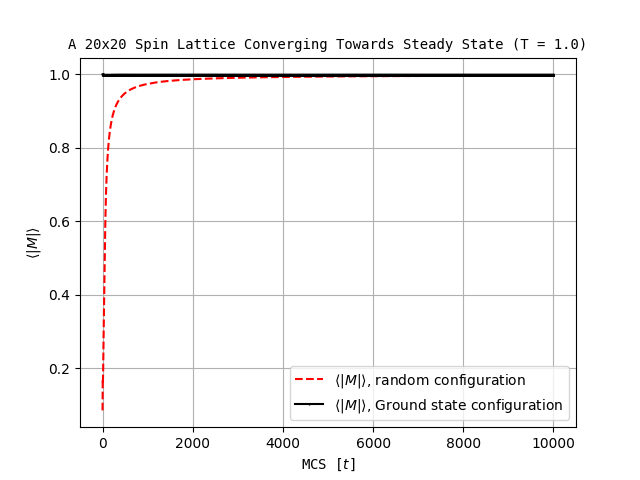
\includegraphics[width=1.08\linewidth]{Figure/20x20_Mconvergence_1.0.png}
			\caption{$k_B T = $ 1.0 J}
		\end{subfigure}
		\begin{subfigure}{0.48\linewidth}
			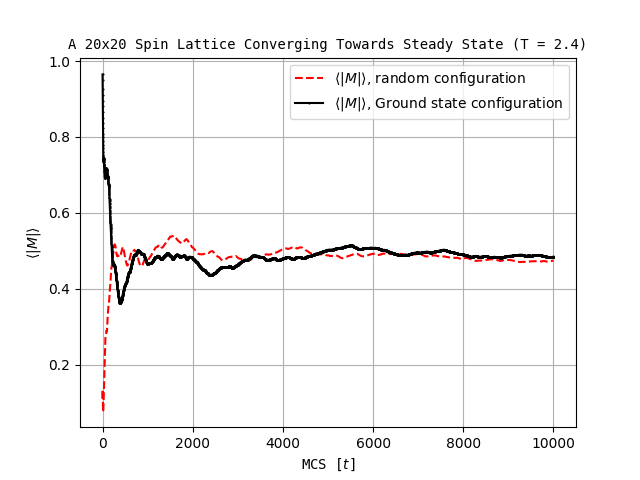
\includegraphics[width=1.08\linewidth]{Figure/20x20_Mconvergence_2.4.png}
			\caption{$k_B T = $ 2.4 J}
		\end{subfigure}
		\caption{Convergence of mean magnetization as a function of Monte Carlo Sweeps (MCS).}
		\label{mconvergence}
	\end{figure}
	
Figure \ref{mconvergence} shows the mean magnetization of systems as function of MCS, for different temperatures and configurations. The trends are mostly the same as the ones seen for the mean energy in Figure \ref{econvergence}.

\begin{figure}[H]
    \centering
    \includegraphics[width = \linewidth]{Figure/accepted_states_in_each_cycle.png}
    \caption{A plot of the acceptance ratio of proposed states as a function of the number of Monte Carlo Sweeps.}
    \label{fig:acceptanceratio}
\end{figure}
Figure \ref{fig:acceptanceratio} is meant to describe the acceptance ratio of proposed states as the algorithm performs several Monte Carlo sweeps through a 20x20 spin lattice. As we see in the leftmost figure, disordered systems at lower temperatures accept very few proposed states after only twenty-some sweeps, indicating the fast convergence towards a steady state. For 'hotter' systems, however, the possibility of accepting proposed states remain significant for a larger number of sweeps. This is also what we may observe in Figure \ref{mconvergence} (b), as the expected mean absolute magnetization fluctuates even after reaching a steady state.\\

\begin{figure}[H]
    \centering
    \includegraphics[width = \linewidth]{Figure/hist_accepted_state.png}
    \caption{Distribution of acceptance ratios for initially disordered systems at temperatures $k_B T = 1.0\ J$ (left) and $k_B T = 2.4\ J$ (right)}
    \label{fig:acceptanceratiodist}
\end{figure}

Figure \ref{fig:acceptanceratiodist} is meant to accompany Figure \ref{fig:acceptanceratio}. From the rightmost figure in Figure \ref{fig:acceptanceratio} it is difficult to tell how a 'hot' disordered system would ever reach a steady state. Considering the distribution of acceptance ratios in a disordered system at $k_B T = 2.4\ J$, we see that there is indeed a good reason as to why such a system would reach a steady state. The probability of accepting proposed states is normally distributed, causing the system to eventually reach a steady state, yet still fluctuate in and out of this state.\\

\begin{figure}[H]
    \centering
    \includegraphics[width = \linewidth]{Figure/distr.png}
    \caption{A plot showing how the energy is distributed at lower temperatures (left) and higher temperatures (right). The $y$ - scales here are not in percent occurrence, rather percent/100. The weighting of the data for the lower temperature lead to wrong $y$-axis scaling. }
    \label{fig:edistr}
\end{figure}

In light of Figure \ref{fig:acceptanceratiodist}, we may also consider how the computed energies are distributed when sweeping through spin lattices at lower and higher temperatures, as we see in Figure \ref{fig:edistr}. In these plots, the distribution of energy in the steady state is shown for two different temperatures. At $k_B T = 1.0 \ J$, the occurrence rate of the ground state energy is much larger than for any other energy, meaning the system rarely deviates from the equilibrium state. For the larger temperature $k_B T = 2.4\ J$ however, we see that although we have reached a steady state, the energies are more widely distributed, supporting the argument that followed from Figure \ref{fig:acceptanceratiodist}, that 'hotter' systems fluctuate in and out of the equilibrium state.\\

\begin{figure}[H]
    \centering
    \includegraphics[width = \linewidth]{Figure/expvals.png}
    \caption{Various plots displaying the temperature dependence of the four physical quantities of interest for different spin lattice dimensions. }
    \label{fig:expvals}
\end{figure}

Figure \ref{fig:expvals} represents the results obtained from running simulations for spin lattices of varying sizes. The top row of the figure shows how the mean energy, and its temperature dependent variance, which we know to be heat capacity, evolves as functions of both temperature and grid size. The bottom row is dedicated to the evolution of the mean absolute magnetization, and its temperature dependent variance, namely magnetic susceptibility. This data was obtained on the temperature interval $T \in [2.0,2.6]$, and with a temperature resolution $\Delta T = 0.005$. In each temperature step, a total of ten million Monte Carlo sweeps were performed. This is by all means a computationally intensive exercise, committing to a run time total of a little over sixteen hours with eight parallel computation processes for the 100x100 spin lattice, and close to twenty hours with four parallel processes for the 80x80 spin lattice. The data obtained for each program execution for different lattice sizes may be found under \texttt{Code/Data} on our GITHUB for reproduction.\\

\begin{table}[H]
\centering
\caption{$T_c$ from the susceptibility for different lattice sizes}
\begin{tabular}{l|l|l}
\hline
Lattice size, L & $T_C$ ($\mathcal{X}$) & $T_C$ ($C_V$)\\
\hline
40 & 2.325 & 2.290\\
60 & 2.305 & 2.290\\
80 & 2.285 & 2.285\\
100 & 2.285 & 2.275\\
\end{tabular}
\label{tab:Tc_susc}
\end{table}
Table \ref{tab:Tc_susc} contains the temperatures at which the data for the magnetic susceptibility $\mathcal{X}$ and the heat capacity $C_V$ has its global maxima for different lattice sizes $\mathcal{L}$. The coordinates $(\mathcal{L}^{-1}, T_C)$ form a data set with which we make a linear model by equation \ref{critical2}. This linear model has an intercept at $\mathcal{L}^{-1} = 0 \to \mathcal{L} = \infty$, which we extract as the critical temperature for an infinitely large spin lattice. 

\begin{figure}[H]
    \centering
    \includegraphics[width = \linewidth]{Figure/figur2.png}
    \caption{Critical temperatures for $C_v$ and $\chi$ for lattices with dimension 40, 60, 80 and 100 have been extracted and plotted. The green graph is the linear regression of the two. The intercept of this graph is at 2.289}
    \label{fig:tcritical}
\end{figure}

By extracting the critical temperatures for $C_v$ and $\chi$ for several lattice dimensions, we have data in which we can utilize the relation in \eqref{critical2}. This is shown in Figure \ref{fig:tcritical}. The intercept point (not shown precisely in the graph, as $\mathcal{L}^{-1} = 0$ is not included in the figure) , which corresponds to $T_C(\mathcal{L}=\infty)$ is at $2.289$.